\documentclass[11pt]{article}

\usepackage{amssymb}
\usepackage{amsmath}
\usepackage{setspace}
\usepackage{graphicx}
\usepackage{subfig}
\usepackage{color}
\usepackage[left=1.2in, right=1in, top=1in, bottom=1in]{geometry}
\usepackage{verbatim}
\usepackage{hyperref}

\begin{document}

\title{Xoptfoil Version 2.01.0 User Guide}
\date{\today}
\maketitle

\tableofcontents

\section{Installing}\label{sec:installing}

\subsection{Linux}\label{sec:build_linux}

Precompiled binaries are not provided for Linux, because it is
generally very easy to get the software required to compile it, and a build script is
provided for convenience. CMake version 2.8.8 or later is required, as are gcc, g++, and
gfortran. Your distribution should have packages for all of these, so locate and install
them first through the package manager.

Once the requirements are installed, all that is necessary should be to run the build script. 
(The build script may not be up to date. If it fails, please report the bug.)
Navigate to the top-level Xoptfoil directory and open a terminal window there. Then, run
the build script using the following command:

\begin{verbatim}
sh build_linux.sh
\end{verbatim}

\noindent or, as long as you have set executable permissions on the script, you can just
use:

\begin{verbatim}
./build_linux.sh
\end{verbatim}

If all goes well, Xoptfoil and its related tools will be installed in linux/bin under the
top-level Xoptfoil directory. If desired, it is possible to change this location by
changing the INSTALLDIR variable in the build script.

You may want to edit your PATH environment variable so that Xoptfoil and its related tools
can be run from any directory. This is done by adding a line to your shell startup script,
normally \$HOME/.bashrc, like the following:

\begin{verbatim}
export PATH=/path/to/Xoptfoil/linux/bin:$PATH
\end{verbatim}

\noindent where the string above is changed to the actual location where Xoptfoil is
installed. A different approach is to install Xoptfoil in a system location, which can be
accomplished most easily by simply removing the line
`-DCMAKE\_INSTALL\_PREFIX:PATH=``\$INSTALLDIR'' \textbackslash' in the build script. The
build script will need to be run with root privileges with this approach. Executables will
then be installed in /usr/local/bin, which should already be in the PATH.

\subsection{Windows}\label{sec:install_windows}

The Windows release includes precompiled binaries of Xoptfoil and its related tools. There
are 64-bit binaries. And only should work on a 64-bit operating system.  The release also
includes some required libraries so that the user does not have to install compilers just
to run Xoptfoil. (The required libraries may not be up to date. If it fails, please report the bug.)
As of Xoptfoil 1.11.0, parallel processing is supported in the
precompiled versions; it is not necessary to compile the code manually to benefit from
this feature.

Currently, the Windows release does not have an official installer; all that is needed is
to unzip the release package and place it somewhere convenient. The executables and
runtime libraries are located in the bin directory. For convenience, it is recommended to
add this directory to the PATH so that Xoptfoil can be executed from other locations. If
you don't do this step, you will need to always run it from the bin directory where the
executables are located or specify the full path when referencing the executables.
To add the Xoptfoil bin directory to your path, on Windows 10:

\begin{enumerate}
  \item{Type ``environment'' in the search box in the task bar.}
  \item{Select ``Edit environment variables for your account.''}
  \item{In the top box, labeled ``Environment variables for $<$user$>$,'' select PATH and
then click EDIT.}
  \item{In the window that appears, add a new entry and then type the location or browse to
the Xoptfoil bin directory. Make sure you do not overwrite any existing entries.}
  \item{Click OK in both windows to save the settings.}
\end{enumerate}

\begin{figure}
\centering
  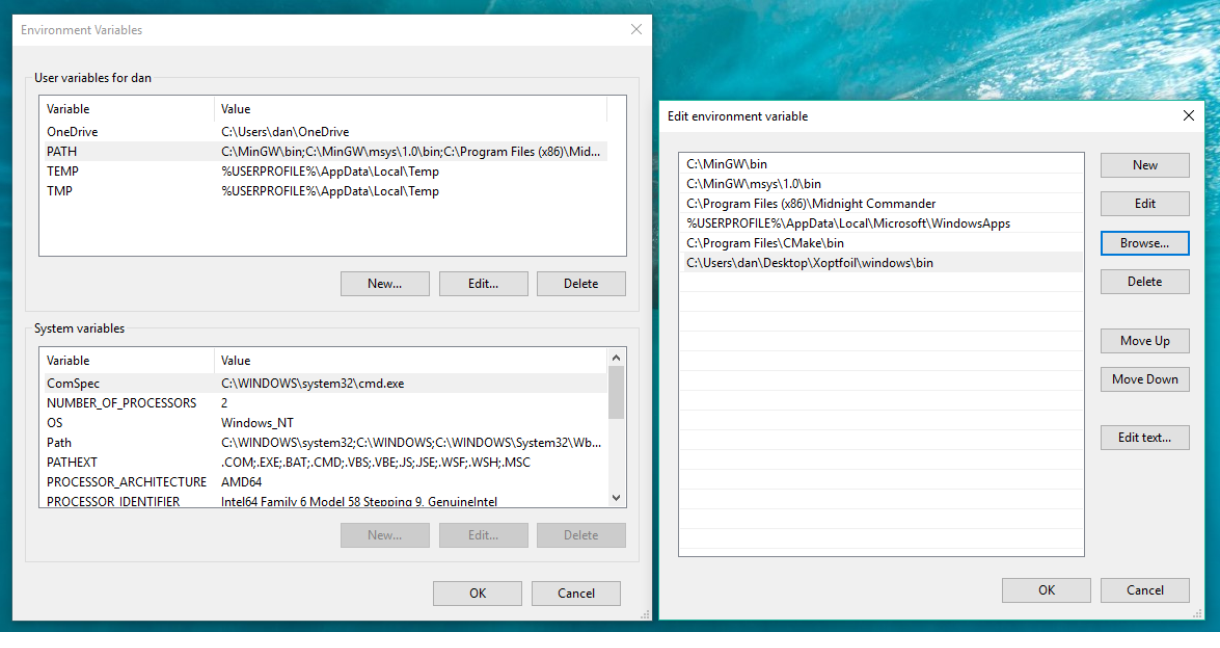
\includegraphics[width=0.85\textwidth]{User_Guide_figs/set_path.png}
\caption{Adding Xoptfoil to the PATH environment \%variable in Windows.}
\label{fig:set_path}
\end{figure}

The two windows should look something like Fig. \ref{fig:set_path}.
On older versions of Windows, the process is similar, but you may need to navigate to the
correct area of the Control Panel to find the environment variable settings, e.g. Control
Panel $\rightarrow$ System $\rightarrow$ Advanced $\rightarrow$ Environment variables. If
you are having trouble finding it, do an internet search for how to set the PATH
environment variable on your version of Windows.

\subsubsection{Optional: compiling}

It is not necessary to compile Xoptfoil on Windows 64-bit, but you are free to do so if desired
(or if you want to make changes to the code). There are a couple prerequesites for
compiling on Windows:

\begin{itemize}
  \item{CMake version 2.8.8 or later, and}
  \item{MinGW32 or MinGW64 including the gcc, g++, and gfortran compilers.}
\end{itemize}

To install CMake, just download and run the installer from the website:
\url{https://cmake.org/download/}. Installing MinGW32 is a little bit more complicated.
The main page for
MinGW is \url{mingw.org}. The installation instructions are at
\url{http://mingw.org/wiki/Getting_Started}. Follow the instructions under the section
``Graphical User Interface Installer'' first. This process will install the MinGW
installation manager, which is a graphical tool used to download and install the MinGW
compilers. In addition to the compilers, you should also install mingw32-make and any
pthreads packages (on MinGW32, these are called mingw32-pthreads-w32). The precompiled
binaries have been built with GCC version 6.3.0 on MinGW32 and 5.4.0 on MinGW64, so these
versions are known to work. MinGW64 can be downloaded at
\url{https://sourceforge.net/projects/mingw-w64/files/mingw-w64/}. However, if your
operating system in 64-bit, MinGW32 should also work fine; you do not need to use MinGW64.
(If MinGW32 fails, please report the bug.)


At this point, everything you need to compile Xoptfoil should be installed. A build script
is provided in the top-level Xoptfoil directory. Though you can run it by double-clicking,
it is recommended to run it from the command line so that the output is visible in case
anything goes wrong. Open a command prompt in that directory browsing there in Windows
explorer, Shift + right-clicking, and selecting ``Open command window here.''
Then, run the build script by entering the following command:

\begin{verbatim}
build_windows.bat
\end{verbatim}

If all goes well, Xoptfoil and its related tools will be installed in
windows{\textbackslash}bin under
the top-level directory.

\subsection{Mac OSX}

To install Xoptfoil on Max OSX, you will need to compile it. (Unfortunately, I don't have a
Mac available to create binaries and do testing.) As with the other platforms, CMake and
a compiler suite are required. CMake is available as a dmg file from the official website:
\url{https://cmake.org/download/}. The GNU compilers are recommended (gcc, g++, and
gfortran), which are available for Mac OSX at
\url{http://gcc.gnu.org/wiki/GFortranBinaries#MacOS}. Because Mac OSX is a Unix-like
system, the build script for Linux should work for Mac OSX as well. Therefore, after
installing CMake and the compilers, you can refer to the Linux compiling instructions in
Section \ref{sec:build_linux} for the rest of the process.

\section{Running Xoptfoil}\label{sec:running}

Xoptfoil is a command-line program. While it is possible to run it by double-clicking on
the executable file, it is better to run it from the command line. (If you double-click to
run it and there is an error, the window will disappear and you won't be able to read the
error message.) Open a terminal
(``command prompt'' in Windows) and navigate to the directory where you intend to run
Xoptfoil. (In the Windows file explorer, you can Shift + right click and select ``Open
command window here.'' Many Linux file browsers have a similar option.)

Note: these instructions assume that you have added the Xoptfoil bin directory where 
binaries are
located to the PATH environment variable as described in Section \ref{sec:installing}.
To run Xoptfoil, simply type the following command:

\begin{verbatim}
xoptfoil
\end{verbatim}

\noindent This command will run Xoptfoil in the current working
directory.  Xoptfoil uses an input file called `inputs.txt,' which must also be in the
working directory.  If the input file is not in the working directory where Xoptfoil is
run, the program will notify you that it can't find the file and then stop. It is also
possible
to use an input file with a different name; see Section \ref{sec:CLOs} for instructions.

By default, Xoptfoil writes output files with the prefix `optfoil' (the final optimized
airfoil is called `optfoil.dat'). However, it is also possible to change the output
prefix, as described in Section \ref{sec:CLOs}.

\subsection{Command line options}\label{sec:CLOs}

Xoptfoil accepts the following command-line options:

\begin{itemize}
  \item{-i \{input file\}
  \begin{itemize}
    \item{Specify an input file other than `inputs.txt.' Replace \{input file\} with the
          name (if in the working directory) or full path to the input file.}
  \end{itemize}}
  \item{-o \{output prefix\}
  \begin{itemize}
    \item{Specify an output prefix other than `optfoil.' Replace \{output prefix\} with the
          desired string.}
  \end{itemize}}
  \item{\texttt{-h, --help}
  \begin{itemize}
    \item{Display usage information and exit.}
  \end{itemize}}
  \item{\texttt{-v, --version}
  \begin{itemize}
    \item{Display Xoptfoil version and license information and exit.}
  \end{itemize}}
\end{itemize}

By way of example, if you wanted to use an input file called `test.txt' and have output
files written with the prefix `my\_airfoil,' you would invoke Xoptfoil with the following
command:

\begin{verbatim}
xoptfoil -i test.txt -o my_airfoil
\end{verbatim}

\section{Controlling an ongoing optimization}\label{sec:run_control}

When Xoptfoil starts an optimization, it creates an empty file called
``run\_control\_\{prefix\}.'' The user can enter commands in this file to control an ongoing
optimization. The currently available commands are:

\begin{itemize}
\item{\textbf{stop}: Write restart data and stop the optimization at the end of the
current iteration. Also writes a stop\_monitoring command, which is described in the next
point.}
\item{\textbf{stop\_monitoring}: In xoptfoil\_visualizer\_V2, stop monitoring the current
optimization and return to the main menu. See Section \ref{sec:xoptfoil_visualizer_V2} for
more information.}
\end{itemize}

\section{Input file}

Xoptfoil reads a Fortran namelist input file called `inputs.txt' (unless a different name
is specified as a CLO, as described above).  This file stores
conditions for optimization, such as the optimization type, parameterization settings,
aerodynamic operating conditions and constraints, the seed airfoil, Xfoil options, etc.
There are a number of categories of inputs, each of which is stored in a separate
namelist.  A Fortran namelist is formatted as follows:

\begin{verbatim}
&namelist_title
  input1 = value1          %Comments are preceeded by a percent sign
  input2 = value2
  textinput1 = `string1'
  etc.
/
\end{verbatim}

Each namelist begins with a `\&' character followed immediately by the title, and it ends with 
a '/' character.  Variables for each namelist are then listed with their respective
values.  To change an input, simply change the value to the right of the `=' sign.  Note
that text-based inputs (for example, the name of the seed airfoil file) need to be
surrounded by single or double quotes. The inputs for each of the Xoptfoil namelists,
stored in `inputs.txt,' are explained in the following sections. A sample input file
called `all\_inputs.txt' is included with Xoptfoil. This file contains all possible
inputs with comments. Many of the inputs are not required, however, and default values
will be used if they are absent. Any absent required inputs will result in an error when
Xoptfoil is run. Any absent namelists will result in an error when Xoptfoil is run.
While running the program, the file echo\_\{prefix\}.txt is created with 
all the options used by Xoptfoil, see Section \ref{sec:output_files} for more information on the
output files generated.

\subsection{optimization\_options namelist}

In this namelist, high-level optimization and parameterization parameters are set.  Each
of the inputs is described in the list below.

\begin{enumerate}
\item{\textbf{search\_type}: May be `global', `local', or `global\_and\_local'.
A global search is an expensive approach like particle swarm or a genetic algorithm which
includes many potential designs to attempt to converge on the global best solution.  A
local search is one that investigates the design space in the vicinity of the initial
design (the seed airfoil), looking for improvements.  A local search is much faster than
a global search, but it also usually does not find as good a final solution.  If this
input is set to `global\_and\_local', a global search is first performed, followed by a
local search.}
\item{\textbf{global\_search}: Optimization algorithm for the global search.  Either
`particle\_swarm' or `genetic\_algorithm'.}
\item{\textbf{local\_search}: Optimization algorithm for the local search.  Currently, the
only available option is `simplex'.}
\item{\textbf{seed\_airfoil}: Defines how to set the seed airfoil.  Available options are
(1) `from\_file', whereby the seed airfoil is read from a file, or (2) `naca', where a
NACA seed airfoil is generated by Xoptfoil. If `naca' is selected, the parameters for
generating the airfoil must be set in the naca\_airfoil namelist. Or (3) `from\_variables',
in which the airfoil is created from the design variables in `airfoil\_file'. It is only available
for `kulfan-bussoletti' and `bezier-parsec' shape functions.}

\item{\textbf{airfoil\_file}: File name for the seed airfoil, which is used if
seed\_airfoil = `from\_file'.  The file must be formatted in Xfoil format; it may have a
label on the first line (though it does not need to) and then the coordinates must be
arranged in two columns for x and y, forming a closed loop beginning and ending at the
trailing edge. There should be no blank lines, and you should also not include the number
of points or any other information besides a header and then the data.  The file must be
in the working directory. Alternatively, if 
seed\_airfoil = `from\_variables', the file must have 3 lines. Two for an header and on 
the third the variables, which must be separated by spaces.}
\item{\textbf{shape\_functions}: Identifier for the shape functions used to parameterize
airfoils in the optimization. A user-defined number of these shape functions are added 
to the top and bottom surfaces of the seed airfoil to create new shapes. These may be:
\begin{enumerate}
	\item `naca', `naca' functions are a family of functions which, when combined in a
	weighted sum, can reproduce many of the NACA airfoils, including four-digit and transonic
	airfoils, on top of the seed airfoil.
	\item `hicks-henne', `hicks-henne' are a more general class of functions which place a ``bump'' of
	variable width and location on the seed airfoil surface.  Each Hicks-Henne shape function,
	therefore, has a strength, a width and a location.
	\item `b-spline', `b-spline' method generates the airfoil solely from the design variables which
	are the coordinates of the control points defining the spline. Two implementations are 
	available, in the first the x coordinate is fixed while on the second it is free, meaning it
	is a design variable. The degree of the spline, the x coordinate distribution and the 
	number of control points must be defined.
	\item `kulfan-bussoletti', `kulfan-bussoletti' also known as class shape functions also
	generates the airfoil solely from the design variables. In this method the design variables
	are the strengths of the functions. An extra strength is available through kulfan\_bussoletti\_LEM.
	\item `bezier-parsec', `bezier-parsec' is similar to the `parsec' parametrization, in here
	the design variables are geometric properties of the airfoil and defined it completely. For 
	this method nfunctions\_top and nfunctions\_bot do nothing since it always has the same number
	of parameters. In order, these are the position of the maximum thickness, the maximum thickness and its curvature,
	the leading edge radius and the trailing edge angle on the thickness. Followed by the the position of the maximum camber, the maximum camber and its curvature, the leading edge camber angle and the trailing edge angle on the camber. 
\end{enumerate}}
\item{\textbf{nparameters\_top}: The number of shape functions used to parameterize the top
	surface of the airfoil.  Note that this number may not correspond to the number of design variables (ndv\_top)
	on the top surface. Instead for:
	\begin{enumerate}
		\item  `naca', nparameters\_top is the number of function therefore $ndv\_top=nparameters\_top$.
		\item `hicks-henne', nparameters\_top is the number of functions therefore $ndv\_top=3 \cdot nparameters\_top$.
		\item `b-spline', nparameters\_top is the number of control points therefore $ndv\_top=nparameters\_top - 2$ if x is fixed or $ndv\_top=2 \cdot nparameters\_top - 5$ if x is free.
		\item `kulfan-bussoletti', nparameters\_top is the order or the degree plus 1, $ndv\_top=nparameters\_top$ without kulfan\_bussoletti\_LEM and $ndv\_top=nparameters\_top + 1$ with it.
		\item `bezier-parsec', nparameters\_top has no meaning and $ndv\_top=5$. 
	\end{enumerate}}
\item{\textbf{nparameters\_bot}: The number of shape functions used to parameterize the
	bottom surface of the airfoil.  See the note on nparameters\_top regarding differences
	between the different shape\_functions.}
\item{\textbf{flap\_optimization\_only}: Whether to optimize only the flap design variables,
	the flap hinge position in x and the flap deflection.}
\item{\textbf{abs\_initial\_perturb}: Generating the initial designs variables requires a maximum and minimum
	value. 
	
	$DV_{max} = DV_{seed} + abs\_initial\_perturb + rel\_initial\_perturb \cdot |DV_{seed}|$
	
	$DV_{min} = DV_{seed} - abs\_initial\_perturb - rel\_initial\_perturb \cdot |DV_{seed}|$
	
	abs\_initial\_perturb controls the absolute increment.}
\item{\textbf{rel\_initial\_perturb}: Generating the initial designs variables requires a maximum and minimum
	value.
	
	$DV_{max} = DV_{seed} + abs\_initial\_perturb + rel\_initial\_perturb \cdot |DV_{seed}|$
	
	$DV_{min} = DV_{seed} - abs\_initial\_perturb - rel\_initial\_perturb \cdot |DV_{seed}|$
	
	rel\_initial\_perturb controls the relative increment.}
\item{\textbf{fla\_optimization\_only}: Whether to optimize only the flap design variables,
	the flap hinge position in x and the flap deflection.}
\item{\textbf{penalty\_limit\_initial}: Initial value of the initial penalty limit. The penalty limit
	controls the maximum penalty value allowed for airfoil evaluation.}
\item{\textbf{penalty\_limit\_end}: End value of the initial penalty limit, the penalty limit follows
	a linear function between initial and end values.}
\item{\textbf{penalty\_factor}: Penalty multipler on objective function.}
\item{\textbf{allow\_seed\_penalties}: Whether the seed airfoil allows for penalties.}
\item{\textbf{min\_bump\_width}: Minimum width of Hicks-Henne bump function.  Too small a
	value is more likely to result in a final design with small ``bumps'' present.  Default
	value is 0.1 (10\% chord).}
\item{\textbf{kulfan\_bussoletti\_LEM}: Wheter to use a adicional design variable for `kulfan-bussoletti'
	shape\_functions to improve the leading edge accuracy, recommended to use.}
\item{\textbf{b\_spline\_degree}: Degree of b-spline curve, used only for `b-spline'
	shape\_functions.}
\item{\textbf{b\_spline\_xtype}: Selects the type of `b-spline' shape\_functions, 1 if x is fixed, 2 if free.}
\item{\textbf{b\_spline\_distribution}: Selects the type of x distribution in `b-spline' shape\_functions, if x
	is free this is the seed distribution. 1 for cossine, 2 for non uniform cossine and 3 for linear.}
\item{\textbf{restart}: Whether or not to restart a prior optimization that terminated
	early -- .true. or .false.  If enabled, files with the pattern restart\_* from the 
	previous run must be present, and most inputs should be kept the same. See Section 
	\ref{sec:restarting} for more information.}
\item{\textbf{restart\_write\_freq}: How often to write restart files, in terms of number
	of iterations.}
\item{\textbf{write\_designs}: Whether to write airfoil coordinates and polars to files
	during the optimization.  See Section \ref{sec:output_files} for more information on the
	output files generated.}
\item{\textbf{write\_cp\_file}: Whether to write cp polar file for designs during the optimization. 
	See Section \ref{sec:output_files} for more information on the output files generated.}
\item{\textbf{write\_bl\_file}: Whether to write bl polar file for designs during the optimization. 
	See Section \ref{sec:output_files} for more information on the output files generated.}
\item{\textbf{write\_dvs\_file}: Whether to write dvs files during the optimization. 
	See Section \ref{sec:output_files} for more information on the output files generated.}
\item{\textbf{number\_threads}: Number of threads to use during optimization.}
\end{enumerate}

\subsection{operating\_conditions namelist}

This namelist specifies aerodynamic operating conditions over which to optimize the
airfoil. These are the operating points at which each potential design will be evaluated,
including angle of attack or lift coefficient, Reynolds number, Mach number, and
relative weighting of each operating point.

\begin{enumerate}
\item{\textbf{noppoint}: The total number of operating points at which to evaluate
	potential designs.  A maximum of 30 is allowed.  Including more operating points makes the
	final design more robust, but there is probably also a point of diminishing returns.
	With only one or two operating points, the final airfoil will
	probably perform quite well at those conditions but do poorly elsewhere.  Including more
	operating points is more expensive, however, because Xfoil must be run for each airfoil at
	each operating point. With many operating points, it is also more likely for Xfoil to not
	converge at one of
	them, which will result in the optimizer essentially throwing out that design.
	Typically, 5 - 10 operating points spanning the range of needed conditions is a
	good number.}
\item{\textbf{use\_flap}: Whether flap deflections will be applied in the optimization.}
\item{\textbf{flap\_connection}: Type of flap connection. Either `sharp', `smooth-top', `smooth-bot' or `smooth'.
	
	`sharp' is the standard connection. A trip wire is added to the sharp point.
	
	`smooth-top' smooths the sharp flap on the top surface from $x\_flap-connection\_radius$ to $x\_flap+connection\_radius$. 
	A trip wire is added to the sharp point if applicable.
	
	`smooth-bot' smooths the sharp flap on the bottom surface from $x\_flap-connection\_radius$ to $x\_flap+connection\_radius$.
	A trip wire is added to the sharp point if applicable.
	
	`smooth' smooths the sharp flap on the both surfaces from $x\_flap-connection\_radius$ to $x\_flap+connection\_radius$.}
\item{\textbf{connection\_apply}: Type of smooth and sharp connections. Either `none', `geometric', `trip\_wire' or `both'.
	
	`none' deactivates the flap\_connection changes.
	
	`geometric' activates the flap\_connection geometric changes.
	
	`trip\_wire' activates the flap\_connection trip wire changes.
	
	`both' activates all the flap\_connection changes.}
\item{\textbf{connection\_radius}: Radius of the smooth connection changes near the plap hinge point in x.}
\item{\textbf{x\_flap\_spec}: Options are `specify' or `optimize'.  In the former case, the input value of x\_flap
	will be used for \textit{all} designs considered by the optimizer.
	In the latter case, the optimizer will consider the flap hinge point in x as a design variable
	and optimize it.  The value of x\_flap will then be used
	only for the seed airfoil to establish the reference seed airfoil performance.}
\item{\textbf{x\_flap}: Flap hinge point in x (between 0 and 1).}
\item{\textbf{y\_flap\_spec}: Method of specifying vertical hinge location. Either `y/c'
	(vertical location normalized by chord length) or `y/t' (vertical location normalized by
	local thickness at x\_flap). The default is `y/c'.}
\item{\textbf{y\_flap}: Flap hinge point in y. Only used if use\_flap is enabled. If
	y\_flap\_spec is `y/c', y\_flap refers to the vertical location of the hinge normalized by
	the chord length. If instead y\_flap\_spec is `y/t', the position is normalized by the
	local thickness at x\_flap. In the latter case, for example, -1.0 places the hinge at the
	lower surface, and 1.0 places it at the upper surface.}
\item{\textbf{TE\_spec}: Options are `use\_seed', `specify' or `optimize'.
	
	`use\_seed', the program uses the seed trailing edge thickness after transformations for all designs.
	
	`specify', the program uses the input value of tcTE for all designs.
	
	 `optimize', the program considers the trailing edge thickness as a design variable
	 and optimize it. The value of tcTE will then be used
	 only for the seed airfoil to establish the reference seed airfoil performance.}
\item{\textbf{tcTE}: Trailing edge thickness.}
\item{\textbf{xltTE}: Starting x position (0 to 1) for seed trailing edge transformation.}

\item{\textbf{op\_mode(n)} (where n is an integer ranging from 1 to noppoint): Tells
	Xfoil whether the angle of attack or lift coefficient is being specified for this
	operating point.  May be `spec-al' for specified angle of attack or `spec-cl' for
	specified lift coefficient.}
\item{\textbf{op\_point(n)} (where n is an integer ranging from 1 to noppoint):
	Specifies either the angle of attack (in degrees) or the lift coefficient for this
	operating point, depending on whether op\_mode is `spec-al' or `spec-cl' for this
	operating point.  Note that Xfoil calculations are not accurate above stall, so do not
	specify too large a lift coefficient or angle of attack.}
\item{\textbf{optimization\_type(n)}: (where n is an integer ranging from 1 to
	noppoint): Specifies the optimization objective for this operating point. Current options 
	include `min-drag' (to minimize drag), `max-glide' (to maximize 
	glide slope), `min-sink' (to minimize sink rate), `max-lift' (to maximize lift at a
	specified angle of attack), `max-xtr' (to move the turbulent transition location as far
	towards the trailing edge as possible), or `max-lift-slope' (to maximize the lift curve
	slope at operating point n).
	
	`target-\{option\}' specifies that the objective is \{options\} value should be target\_value. 
	With \{option\} = \{lift, drag, moment, xtrt, xtrb, glide or sink\}.
	
	`max-lift-search' maximizes the lift in a interval set by op\_point\_start, op\_point\_end and op\_point\_step.}
\item{\textbf{use\_previous\_op(n)} (where n is an integer ranging from 1 to noppoint): Whether to use previous op polar results.
	Allows for optimization of different objectives for the same operating point without increasing the number of XFOIL analysis.}

\item{\textbf{op\_point\_start(n)} (where n is an integer ranging from 1 to noppoint): Start value for op\_point(n) interval in `max-lift-search' in optimization\_type(n).}

\item{\textbf{op\_point\_end(n)} (where n is an integer ranging from 1 to noppoint): End value for op\_point(n) interval in `max-lift-search' in optimization\_type(n).}

\item{\textbf{op\_point\_step(n)} (where n is an integer ranging from 1 to noppoint): Step value for op\_point(n) interval in `max-lift-search' in optimization\_type(n).}

\item{\textbf{target\_value(n)} (where n is an integer ranging from 1 to noppoint): Target value for `target-\{option\}' in optimization\_type(n).}

\item{\textbf{reynolds(n)} (where n is an integer ranging from 1 to noppoint): Specifies
	the Reynolds number based on chord for this operating point.}
\item{\textbf{mach(n)} (where n is an integer ranging from 1 to noppoint): Specifies
	the Mach number for this operating point.  Note that Xfoil calculations are not accurate
	at or above the transonic regime, so do not specify too high a Mach number.}

\item{\textbf{flap\_selection(n)} (where n is an integer ranging from 1 to noppoint):
	Options are `specify', `identical' or `optimize'.  
	
	For `specify', the input value of flap\_degrees(n)
	will be used at this operating point for \textit{all} designs considered by the optimizer.
	
	For `identical', flap\_degrees(n) uses the value from flap\_degrees(flap\_identical\_op(n)).
	
	For `optimize', the optimizer will consider the flap deflection as a design variable
	and optimize it at this operating point.  The value of flap\_degrees will then be used
	only for the seed airfoil to establish the reference seed airfoil performance.}
\item{\textbf{flap\_identical\_op(n)} (where n is an integer ranging from 1 to noppoint):
	Operating point number used for `identical' flap\_selection(n).}

\item{\textbf{flap\_degrees(n)} (where n is an integer ranging from 1 to noppoint):
	Specifies the flap deflection for this operating point, in degrees, with a positive
	deflection being in the downward direction. Only used if use\_flap is enabled. The
	optimized flap deflection is subject to the constraints max\_flap\_degrees and
	min\_flap\_degrees.}
\item{\textbf{weighting(n)} (where n is an integer ranging from 1 to noppoint): Specifies
	the weighting for this operating point.  Operating points with a higher weighting are
	given more importance by the optimizer.  Note that the weightings are automatically 
	normalized by the optimizer so that they add up to 1.}
\item{\textbf{ncrit\_pt(n)} (where n is an integer ranging from 1 to noppoint): Specifies
	ncrit for this operating point. If not specified, the ncrit value from the
	xfoil\_run\_options namelist will be used.}
\end{enumerate}

\subsection{constraints namelist}

Specifies aerodynamic and geometric constraints for the optimization.  Constraints are
implemented in the optimizer by assigning a large penalty value whenever a constraint is
violated.

\begin{enumerate}
\item{\textbf{min\_thickness}: The minimum allowable thickness of designs, as a
fraction of the chord (for example, 0.08 means 8\% thickness).  A minimum allowable
thickness is usually required for structural reasons.  If you don't want to impose this
constraint, just set it to 0.}

\item{\textbf{max\_thickness}: The maximum allowable thickness of designs, as a
fraction of the chord (for example, 0.08 means 8\% thickness). This can be used to set an
upper bound on max airfoil thickness.  If you don't want to use this constraint, just set
it to a very large number like 1000 (or just don't specify a max\_thickness, as 1000 is
the default value).}

\item{\textbf{min\_camber}: The minimum allowable camber of designs, as a fraction of the
chord (for example, 0.02 means 2\% camber). If you don't want to impose this constraint,
set it to some large negative value (the default is -0.10).}

\item{\textbf{max\_camber}: The maximum allowable camber of designs, as a fraction of the
chord (for example, 0.02 means 2\% camber). If you don't want to impose this constraint,
set it to some large positive value (the default is 0.10).}

\item{\textbf{symmetrical} (.true. or .false.): Whether to only generate symmetrical 
	airfoils.  If true, only the top surface of the seed airfoil will be modified, and the
	bottom surface will be replaced by a mirrored version of the top surface. This option is
	useful if you want to ensure that the final optimized airfoil is symmetrical.  The seed 
	airfoil does not need
	to be symmetrical to use this option (but note that Xoptfoil will actually be using a
	symmetrical version of the seed airfoil instead of the actual one).}

\item{\textbf{max\_growth\_seed\_mult}: Largest allowable growth rate multipler on seed max growth rate. 
	If you don't want to impose this constraint, just set it to a high value.}

\item{\textbf{min\_leading\_edge\_angle}: Lowest allowable value of leading edge angle. 
	If you don't want to impose this constraint, just set it to 0.}
\item{\textbf{max\_leading\_edge\_angle}: Largest allowable growth rate multipler on seed max growth rate. 
	If you don't want to impose this constraint, just set it to a high value.}
\item{\textbf{dif\_leading\_edge\_angle}: Largest allowable value of leading edge angle 
	difference between top and botton. 
	If you don't want to impose this constraint, just set it to a high value.}

\item{\textbf{min\_te\_angle}: The minimum trailing edge wedge angle, in degrees.  Without
	this constraint, the optimizer may converge on airfoils with a very thin cusped aft
	section, which is challenging to build and presents structural problems.  If you don't
	want to impose this constraint, just set it to 0.}
\item{\textbf{te\_angle\_x\_apply}: The starting x position in which to apply min\_te\_angle constrain.}

\item{\textbf{max\_panel\_angle}: Largest allowable value of panel angle. 
	If you don't want to impose this constraint, just set it to a high value.}

\item{\textbf{lift\_check\_tol}: Lift tolerance before checking at a perturb point. 
	If you don't want to impose this constraint, just set it to a high value.}
\item{\textbf{drag\_check\_tol}: Drag tolerance before checking at a perturb point. 
	If you don't want to impose this constraint, just set it to a high value.}

\item{\textbf{max\_flap\_degrees}: Maximum flap angle, in degrees, for `optimize' flap 
	selection type in operating\_conditions, where positive corresponds to a downward
	deflection.}

\item{\textbf{min\_flap\_degrees}: Minimum flap angle, in degrees, for `optimize' flap 
selection type in operating\_conditions, where positive corresponds to a downward
deflection.}

\item{\textbf{max\_flap\_x}: Maximum flap hinge position in x for `optimize' flap 
	selection type in operating\_conditions.}

\item{\textbf{min\_flap\_x}: Minimum flap hinge position in x for `optimize' flap 
	selection type in operating\_conditions.}

\item{\textbf{max\_tcTE}: Maximum trailing edge thickness for `optimize' flap 
	selection type in operating\_conditions.}

\item{\textbf{min\_tcTE}: Minimum trailing edge thickness for `optimize' flap 
	selection type in operating\_conditions.}

\item{\textbf{check\_curvature}: Whether to check the curvature for applying a curvature
reversals constraint.  If you don't want to apply a curvature reversals constraint, set
this to .false., because checking the curvature adds computational cost.  Set this to
.true. if you wish to specify a constraint on the number of curvature reversals.}

\item{\textbf{max\_curv\_reverse\_top}: Maximum allowed number of curvature reversals on
the top surface within the specified curvature threshold.  If you wish to use this 
constraint, you must enable check\_curvature. The default is 0. Increasing it may improve
the predicted performance but also may produce more wavy designs.}

\item{\textbf{max\_curv\_reverse\_bot}: Maximum allowed number of curvature reversals on
the bottom surface within the specified curvature threshold.  If you wish to use this 
constraint, you must enable check\_curvature. The default is 1, so a single curvature
reversal is allowed on the bottom surface.  Increasing it may improve the predicted
performance but also may produce more wavy designs.}

\item{\textbf{curv\_threshold}: Curvature thresshold for detecting reversals.  The local
curvature can be thought of as 1/r, where r is the local radius.  So, for instance, a
curvature threshold of 0.2 means that any reversals with a radius greater than 5.0 will
be ignored.  If you make this value too small, it may be very hard for the optimizer to
come up with feasible designs, so you may need to increase feasible\_init\_attempts. The
default is 0.1.} 


\item{\textbf{moment\_constraint\_type(n)} (where n is an integer ranging from 1 to
	noppoint): How to implement the pitching moment constraint for the specified operating
	point. Either `none', `specify', or `use\_seed'.  If `none', then no pitching moment 
	constraint is applied at this operating point.  If `specify', then the user specifies the 
	minimum allowable moment using the min\_moment constraint.  If `use\_seed', then the 
	pitching moment from the seed airfoil at this operating point will be taken as the minimum
	allowable.}

\item{\textbf{min\_moment(n)} (where n is an integer ranging from 1 to noppoint): The 
	minimum allowable pitching moment coefficient at the specified operating point.  A larger
	negative pitching moment will require a larger tail.  For flying-wing airfoils, this is 
	usually set to 0.  This input is only used if moment\_constraint\_type = `specify'.} 

\item{\textbf{lift\_constraint\_type(n)} (where n is an integer ranging from 1 to
	noppoint): How to implement the lift constraint for the specified operating
	point. Either `none', `specify', or `use\_seed'.  If `none', then no lift 
	constraint is applied at this operating point.  If `specify', then the user specifies the 
	minimum allowable lift using the min\_lift constraint.  If `use\_seed', then the 
	lift from the seed airfoil at this operating point will be taken as the minimum
	allowable.}

\item{\textbf{min\_lift(n)} (where n is an integer ranging from 1 to noppoint): The 
	minimum allowable lift coefficient at the specified operating point.} 

\item{\textbf{drag\_constraint\_type(n)} (where n is an integer ranging from 1 to
	noppoint): How to implement the drag constraint for the specified operating
	point. Either `none', `specify', or `use\_seed'.  If `none', then no drag 
	constraint is applied at this operating point.  If `specify', then the user specifies the 
	maximum allowable drag using the min\_lift constraint.  If `use\_seed', then the 
	drag from the seed airfoil at this operating point will be taken as the maximum
	allowable.}

\item{\textbf{max\_drag(n)} (where n is an integer ranging from 1 to noppoint): The 
	maximum allowable drag coefficient at the specified operating point.} 

\item{\textbf{naddthickconst}: Number of additional thickness constraints to specify. The
max allowed is 10.}

\item{\textbf{addthick\_x(n)} (where n is an integer ranging from 1 to naddthickconst):
x/c location where additional thickness constraint n is applied.}

\item{\textbf{addthick\_min(n)} (where n is an integer ranging from 1 to naddthickconst):
The minimum thickness allowed at the location specified by addthick\_x(n).}

\item{\textbf{addthick\_max(n)} (where n is an integer ranging from 1 to naddthickconst):
The maximum thickness allowed at the location specified by addthick\_x(n).}
\end{enumerate}

\subsection{naca\_airfoil namelist}

This namelist specifies options for generation of a NACA airfoil, which are used if 
seed\_airfoil = `naca' in the optimization\_options namelist. NACA airfoil generation is
provided by the naca456 code from \url{http://www.pdas.com}, which has been adapted for
Xoptfoil. Instead of specifying a 4-, 5-, or 6-digit code with limited precision, most
inputs are supplied as real numbers, which allows greater precision (e.g., you can create
a 4-digit airfoil with 2.5\% camber). However, be aware that some families are only
intended to be used with specific ranges of these inputs, and setting a parameter too
large or small may result in an unexpected shape. This mainly true of the 4M and 5
families. Therefore, the user should do some research first to see what ranges are
allowed.

\begin{enumerate}
\item{\textbf{family}: NACA airfoil family. Options are `4', `4M', `5', `63', `64', `65',
`66', `67', `63A', `64A', or `65A'.}
\item{\textbf{maxt}: Max thickness as a fraction of chord. For example, for a 10\%-thick
airfoil, use maxt = 0.10.}
\item{\textbf{xmaxt}: Location of maxt as a fraction of chord. This input is only used for
the 4M family.}
\item{\textbf{maxc}: Max camber as a fraction of chord. For example, for 2\% camber, use
maxc = 0.02. This input is only used for the 4 and 4M families (others use design\_cl 
instead to adjust the camber).} 
\item{\textbf{xmaxc}: Location of maxc as a fraction of chord.}
\item{\textbf{design\_cl}: Design lift coefficient. This input is only used for the 5, 6,
and 6A families.}
\item{\textbf{a}: Extent of constant load for the 6 family. It is specified as a fraction
of chord.}
\item{\textbf{leidx}: Leading edge index for the 4M family.}
\item{\textbf{reflexed} (.true. or .false.): Whether the mean camber line is reflexed.
This input is only used for the 5 family.}
\end{enumerate}

\subsection{initialization namelist}

This namelist specifies options for initialization a population of designs for the global
search methods (particle swarm and genetic algorithm).

\begin{enumerate}
\item{\textbf{feasible\_init} (.true. or .false.): If true, attempts to place initial
designs in the feasible space.  If an initial design violates constraints, a large penalty
value will be added to the objective function.  feasible\_init will re-randomize
designs that initially have too large an objective function value.  
This process increases the overall expense of the optimization but also improves the 
results because more of the initial designs will be good ones.}
\item{\textbf{feasible\_limit}: The objective function value below which initial
designs are considered feasible.  Designs that violate constraints are added a penalty
value on the order of $10^6$, so the feasible limit should be large but at least an order
of magnitude smaller than $10^6$.  The default value is 50,000.}
\item{\textbf{feasible\_init\_attempts}: Number of attempts to try to make an initial
design feasible.  The default is 1000. This number is usually sufficient to get most or
all of the designs in the feasible space.  However, if many of the designs cannot be made
feasible within 1000 attempts, you should increase the number. (This may happen if very
tight geometric constraints are applied.)}
\end{enumerate}

\subsection{particle\_swarm\_options namelist}

This namelist specifies options for particle swarm optimization, which are used if
search\_type = `global' or search\_type = `global\_and\_local' and global\_search =
`particle\_swarm'.

\begin{enumerate}
\item{\textbf{pso\_pop}: Number of particles.  These are randomly initialized throughout 
the design space and then use swarming behavior to converge on the global optimimum.  
Search cost increases linearly with population size.  Usually, around 40 or 50 particles 
seem to work well.}
\item{\textbf{pso\_tol}: Tolerance in max radius of particles before triggering a stop
condition.  When all particles are within this radius of the population center, the
particle swarm optimization process will stop even if the max number of iterations has
not been reached. The default value is 0.0001.}
\item{\textbf{pso\_maxit}: Maximum number of iterations allowed before the particle swarm
optimization is stopped.  The default value is 700.  Using the 
`quick' convergence profile, the optimization will usually converge in less than 700
iterations. However, if you use the `exhaustive' profile, it likely will not converge
within the default 700 iterations, but the airfoil design will probably not improve much 
after that.}
\item{\textbf{pso\_convergence\_profile}: Either `exhaustive' or `quick'.  This setting
adjusts some parameters in the particle swarm algorithm which affect how quickly the
optimization converges.  The quick profile works well and converges quickly.  The
exhaustive profile usually is able to find a little bit better designs than the quick
profile, but it also takes much longer to converge (e.g., 700 iterations instead of 150).}
\item{\textbf{pso\_speed\_limit}: Speed limit value, default value is 0.025.}
\end{enumerate}

\subsection{genetic\_algorithm\_options namelist}

This namelist specifies options for genetic algorithm optimization, which are used if
search\_type = `global' or search\_type = `global\_and\_local' and global\_search =
`genetic\_algorithm'.

\begin{enumerate}
\item{\textbf{ga\_pop}: Number of designs in the population.  These are randomly
initialized throughout the design space and then use reproduction and replacement
mechanisms to converge on the global optimum.  Search cost increases linearly with
population size, as long as \textbf{parent\_fraction} remains the same.  Usually, around
80 to 100 particles seem to work well.}
\item{\textbf{ga\_tol}: Tolerance in max radius of designs before triggering a stop
condition.  When all designs are within this radius of the population center, the
genetic algorithm optimization process will stop even if the max number of iterations has
not been reached.  The default value is 0.0001. Note: not all designs are considered in
the design radius computation.  Only the best nparents designs, where nparents is the
number of designs that reproduce during each iteration, are considered.  This is because
the worst designs are typically less likely to reproduce (unless
\textbf{parents\_selection\_method} is `random') and may take a long time to move
towards the optimum.}
\item{\textbf{ga\_maxit}: Maximum number of iterations allowed before the genetic
algorithm optimization process is stopped.  The default value is 700.  It is likely that
the optimization process will not converge within the default 700 iterations, but the
airfoil design will probably not improve much after that.}
\item{\textbf{parents\_selection\_method}: Method of selecting parents during each
iteration.  Available options are `roulette', `tournament', or `random'.  The first two
are usually best.  The default is `tournament'.}
\item{\textbf{parent\_fraction}: Fraction of the total population that reproduces during
each iteration. The default is 0.5.}
\item{\textbf{roulette\_selection\_pressure}: Factor to increase the likelihood that the
best designs are selected as parents when using the roulette parent selection method.  The
default value is 8.0.}
\item{\textbf{tournament\_fraction}: Fraction of the total population that is randomly
entered into the tournament for selecting parents designs, when
\textbf{parents\_selection\_method} is `tournament'.  For example, if
\textbf{tournament\_fraction} is 0.1 and \textbf{ga\_pop} is 100, then 10 designs will be
randomly selected, and the parent will be the best of these 10 designs.  (This process is
repeated for each parent that is selected.)}
\item{\textbf{crossover\_range\_factor}: If 0, crossover will result in design variables
that are linear interpolations between parents.  A value greater than 0 allows
extrapolation to occur, which is recommended to ensure that the design space is adequately
searched.  The default value is 0.5, which means crossover can result in design variables
that are 50\% in excess of the difference in the parent values in either direction.}
\item{\textbf{mutant\_probability}: The probability of mutation occurring in a given
offspring.  The default is 0.4, which means that there is a 40\% probability that a given
offspring design will be able to mutate.}
\item{\textbf{chromosome\_mutation\_rate}: For mutant designs, the probability that a
given design variable (a.k.a. chromosome) will mutate. This should be small enough to not
pollute the ``genes'' of good designs, but large enough that variation is introduced in
the gene pool.  The default is 0.01, which means that 1\% of the design variables will
mutate in child designs that are flagged for mutation.}
\item{\textbf{mutation\_range\_factor}: Maximum magnitude of mutation, as a fraction of
the initially specified design variable range.  For shape design
variables, this range is defined by initial\_perturb, and for flap design variables the
range is the difference between the max and min flap angles.  The default value is 0.2, or
20\% of the range.}
\end{enumerate}

\subsection{simplex\_options namelist}

This namelist specifies options for simplex optimization, which are used if
search\_type = `local' or search\_type = `global\_and\_local' and local\_search =
`simplex'.

\begin{enumerate}
\item{\textbf{simplex\_tol}: Tolerance in max radius of designs before triggering a
stopping condition.  When all designs are within this radius of the simplex center, the
simplex optimization process will stop even if the max number of iterations has not been
reached.  The default value is 10$^{-6}$.}
\item{\textbf{simplex\_maxit}: Maximum number of iterations allowed before the simplex
optimization is stopped.  Ensures that the simplex optimization does not go on for
too long before the stopping condition is met.}
\end{enumerate}

\subsection{xfoil\_run\_options namelist}

This namelist specifies options that control how Xfoil calculations are run.

\begin{enumerate}
\item{\textbf{ncrit}: Transition-triggering parameter.  A higher number represents cleaner
(less turbulent) freestream conditions.  9 is the default.}

\item{\textbf{xtript}: Top-surface trip location for turbulent transition.  For free
transition, set this to 1.  1 is the default.}

\item{\textbf{xtripb}: Bottom-surface trip location for turbulent transition.  For free
transition, set this to 1.  1 is the default.}

\item{\textbf{viscous\_mode} (.true. or .false.): Whether to run Xfoil boundary layer
calculations.  The default is .true., which is recommended.  If it is .false., the pressure
drag is used as the drag coefficient, which isn't very meaningful for real designs.}

\item{\textbf{silent\_mode} (.true. or .false.): If .true., suppresses Xfoil screen writes.
This is desirable for optimization, because thousands of designs are tested and there is
not time to read the Xfoil notifications anyway.  For running Xfoil alone without
optimizing, you may want to see the Xfoil screen writes.  .true. is the default.}

\item{\textbf{bl\_maxit}: Max number of iterations for viscous calculations.  100 is the
default.}

\item{\textbf{vaccel}: Xfoil viscous convergence acceleration parameter.  0.01 is the
default.}

\item{\textbf{reinitialize} (.true. or .false.): Whether to reinitialize the boundary
	layer at each consecutive operating point.  .true. is the default, which seems to result 
	in a more robust optimization, but you may want to experiment with this.}


\item{\textbf{init\_type}: Either `always', `unconverged' or `never'.
	This setting sets how a operating point is analyzed in XFOIL.
	
	`always' sets that the operating should be approached through a sequential analysis of a initializing polar.
	
	`unconverged' sets that the operating should analyzed normally. However if it unconverges the point will be reanalyzed through a sequential analysis of a initializing polar.
	
	`never' sets that the operating should analyzed normally, regardless of convergence.}

\item{\textbf{init\_number\_points} Number of points in the initializing polar.}
\item{\textbf{init\_al0} Angle of attack reference value for initializing polar.}
\item{\textbf{init\_cl0} Lift coefficient reference value for initializing polar.}
\item{\textbf{init\_initial\_position} Adimensional start position in initializing polar. With 0 being the reference value and 1 being the operating point.}
\item{\textbf{init\_dist} Distribution of initializing polar points. Either `linear' or `sine'.}
\end{enumerate}

\subsection{xfoil\_paneling\_options namelist}

This namelist controls how Xfoil smooths airfoil paneling before running aerodynamic
calculations.  The options are the same as the PPAR menu in Xfoil.

\begin{enumerate}
\item{\textbf{npan}: Number of airfoil panels.}
\item{\textbf{cvpar}: Panel bunching parameter.  Increasing this number will cause more
panels to be bunched in regions of high curvature. 1.0 is the default.}
\item{\textbf{cterat}: Ratio of trailing-edge to leading-edge panel density.  0.15 is the
default.}
\item{\textbf{ctrrat}: Ratio of regular panel density to refined-area panel density.  0.2
is the default.}
\item{\textbf{xsref1}: Left top side refinement limit.  1.0 is the default, which means
there is no refined area on the top side.}
\item{\textbf{xsref2}: Right top side refinement limit.  1.0 is the default.}
\item{\textbf{xpref1}: Left bottom side refinement limit.  1.0 is the default, which means
there is no refined area on the top side.}
\item{\textbf{xpref2}: Right bottom side refinement limit.  1.0 is the default.}
\end{enumerate}

\subsection{matchfoil\_options namelist}

This namelist is used for testing new optimization algorithms and parameterization
schemes.  Instead of running an aerodynamic optimization (which is expensive), this
namelist allows you to try to match the seed airfoil shape to another known airfoil shape,
and Xfoil is never run.  It's about a million times faster than aerodynamic optimization
(rough estimate), which makes it good for testing things.

\begin{enumerate}
\item{\textbf{match\_foils} (.true. or .false.): If .true., the optimizer will try to
match the seed airfoil shape to another known airfoil shape, and no aerodynamic
calculations will be performed.  .false. is the default.}
\item{\textbf{match\_foil\_file}: Text string specifying the file name of the airfoil
which is to be matched by the optimizer.  The coordinates must be given in Xfoil format,
meaning the first line can be a label (but it doesn't have to be), and then the x and y
coordinates must follow in two columns arranged in a single loop beginning and ending at
the trailing edge. If the file is not in the working directory, you must include the
relative path.}
\end{enumerate}

\section{Output files}\label{sec:output_files}

The following files are written out by the program. By default, \{prefix\} is ``optfoil,''
unless otherwise specified with the -o command line option as described in Section
\ref{sec:CLOs}.

\begin{enumerate}
\item{\textbf{echo\_\{prefix\}.txt}: File with the inputs used in the program. Can be read by xoptfoil.}

\item{\textbf{seed\_\{airfoil\_file\}}: File with the airfoil coordinates after transformations (scaling, rotating and translating).}

\item{\textbf{TE\_seed\_\{airfoil\_file\}}: File with the airfoil coordinates after trailing edge transformation.}

\item{\textbf{param\_seed\_\{airfoil\_file\}}: File with the airfoil coordinates after being parametrized.}


\item{\textbf{\{prefix\}.dat}: The coordinates of the final optimized design.}

\item{\textbf{\{prefix\}\_performance\_summary.dat}: Aerodynamic data for the final optimized
design at the requested operating points.}

\item{\textbf{\{prefix\}\_optimization\_history.dat}: Convergence information from the optimizer,
	including the iteration, objective function value of the best design, percent improvement
	over the seed airfoil, and radius of the candidate designs. This information can be
	plotted using xoptfoil\_visualizer\_V2; see Section \ref{sec:xoptfoil_visualizer_V2} for more
	information.}

\item{\textbf{\{prefix\}\_design\_coordinates.dat}: Airfoil coordinates for each
progressively better design found during the optimization.  Only written if the option
write\_designs is set to .true.  Each new design is identified under one of the ``zone
t=...'' labels.  You can plot these using xoptfoil\_visualizer\_V2. See Section 
\ref{sec:xoptfoil_visualizer_V2} for more information.}

\item{\textbf{\{prefix\}\_design\_polars.dat}: Airfoil polars (lift, drag, pitching
moment coefficients, and transition locations) at
the requested operating points for each progressively better design found during the 
optimization.  Only written if the option write\_designs is set to .true.  Each new design
is identified under one of the ``zone t=...'' labels.  You can plot these using 
xoptfoil\_visualizer\_V2. See Section \ref{sec:xoptfoil_visualizer_V2} for more information.}

\item{\textbf{\{prefix\}\_design\_aifoil\_variables.dat}: Airfoil design variables file for the
	last design.}


\item{\textbf{A number of files with the pattern restart\_*\_\{prefix\}}: Restart data
written by Xoptfoil.  These files are required to restart a prior optimization that was
terminated early. More information is available in Section \ref{sec:restarting}.}

\item{\textbf{run\_control\_\{prefix\}}: File that allows control over optimization stop and monitoring stop in 
	xoptfoil\_visualizer\_V2.}

\item{\textbf{dvs\_*\_\{prefix\}.dat}: File that saves all design variables, objective value and return type.}
\item{\textbf{aero\_*\_\{prefix\}.dat}: File that saves all objective variables.}
\item{\textbf{constrain\_*\_\{prefix\}.dat}: File that saves all constrain variables.}
\end{enumerate}

\section{Restarting an optimization}\label{sec:restarting}

Because Xoptfoil can take several hours to optimize an airfoil design, sometimes it is
desirable to terminate an optimization early and pick up again later. Terminating an
ongoing optimization may be done by entering the ``stop'' command in the run\_control
file. Xoptfoil can restart a prior optimization
by reading restart files that are written periodically. The file
restart\_status\_\{prefix\}
saves the current optimization method being used, either global optimization (i.e.,
particle swarm) or local optimization (simplex).  The file restart\_pso\_\{prefix\} contains
data required by the particle swarm optimizer to restart a prior optimization. Similarly,
the file restart\_ga\_\{prefix\} contains restart data for the genetic algorithm,
and restart\_simplex\_\{prefix\} contains restart data for the simplex search.
Each of these files must be
present in the working directory when Xoptfoil is run in order to restart properly.

The two relevant inputs are \textbf{restart} and \textbf{restart\_write\_freq} in the
optimization\_options namelist.  For a new optimization, \textbf{restart} should be set to
.false., but it must be .true. to restart a prior optimization.
\textbf{restart\_write\_freq} specifies how often restart data is written to files, in
terms of iterations.  Other than \textbf{restart}, the rest of the inputs should be the
same when restarting an optimization.  However, it is possible to also change any settings
that do not affect the number of design variables or population of designs and still
restart successfully.  For example, Xfoil paneling and run options can be changed when
restarting, but the number of operating points cannot. 

\section{Using xoptfoil\_visualizer\_V2}\label{sec:xoptfoil_visualizer_V2}

A Python script called xoptfoil\_visualizer\_V2.py is provided to plot and animate airfoil
designs generated during the optimization process, either while the optimization is going
on or afterwards.  In order to use this tool, it is
necessary to have Python with matplotlib and numpy installed. It has been tested with
Python 2.7.x and Python 3.6.x, and matplotlib version 1.5.0 or higher is recommended.
On Windows, the easiest
way to achieve this is to install one of the free packaged Python distributions.  The
Anaconda Python distribution is recommended because it is easy to install and includes
up-to-date versions of all the required packages.  Anaconda can be downloaded here:
\url{https://www.continuum.io/downloads}.

When installing Anaconda (or whichever Python distribution is chosen), be sure to check
the option to add Python to your PATH.  That way, Python can be run from the
command prompt.  If you are not using Anaconda and the option to modify the system path is
not offered, you should manually add the appropriate directory with the python executable
to your path, following a similar method to the one described in Section
\ref{sec:install_windows} where the Xoptfoil bin directory was added to the path.

If you are using Linux, it is likely that you already have Python installed on your
system.  However, matplotlib may not be installed by default; if so, install it from your
distribution's software repository.  Note that there may be different packages for 
matplotlib
and numpy depending on whether you are using Python 2 or Python 3. Again, matplotlib
version 1.5.0 or higher is recommended.

To use xoptfoil\_visualizer\_V2, you must first start an optimization with write\_designs set
to .true. In the same directory, run xoptfoil\_visualizer\_V2 using the following command:

\begin{verbatim}
xoptfoil_visualizer_V2.py
\end{verbatim}

Note that xoptfoil\_visualizer\_V2.py must be present in the directory where you try to run it,
or it must be in your PATH environment variable as described in Section
\ref{sec:installing}. xoptfoil\_visualizer\_V2 is menu based.  When it is run, 
it first asks for the case name of the optimization.  By default, this is `optfoil,' but
it will be different if you specified a different name as a command line argument to
xoptfoil. (It is the prefix in front of the files 
\{prefix\}\_design\_coordinates.dat and
\{prefix\}\_design\_polars.dat.)  The prompt looks like this:

\begin{verbatim}
Enter the case name for the optimization (e.g., optfoil, which 
is the default case name): 
\end{verbatim}

After specifying the case name, the tool will attempt to read the files.  Provided they
are present, the number of designs read from them will be printed to screen, and then the
main menu will be shown.  The following shows an example status notification for reading
files with the case name `optfoil' (the default), and below it the menu:

\begin{verbatim}
Reading airfoil coordinates from file optfoil_design_coordinates.dat...
Found 52 airfoil coordinates plus seed airfoil.
Reading airfoil polars from file optfoil_design_polars.dat...
Found 52 airfoil polars plus seed airfoil.

Options:
[0] Exit
[1] Plot a specific design
[2] Animate all designs 
[3] Monitor an ongoing optimization
[4] Change plotting options

Enter a choice [0-4]: 
\end{verbatim}

Option 1 will offer you the choice to plot any of the airfoils and polars that were
generated during the optimization. It also will show the optimization history if that
output file is present. Option 2 creates the same plots (except for the optimization 
history), but it loops through all the designs and displays them in sequence. Option 3 is
similar to option 2, except that it is used to monitor the results of an ongoing
optimization. When this option is selected, the output files from Xoptfoil are checked at
a regular interval, and the plots are updated automatically when new data is available. 
Monitoring can be stopped by entering the command ``stop\_monitoring'' (without quotes) on
a new line in the run\_control file, as described in Section \ref{sec:run_control}.
Plotting options can be 
changed by selecting option 4.  Available plotting options include turning on/off various
plot elements (such as the seed airfoil, the coordinate  plot, and the polar plot), line 
colors, and the checking interval when monitoring an ongoing optimization.  The plotting 
options menu also allows animation frames to be saved. When this option is enabled and 
option 2 is selected from the main menu, each frame of the animation will be saved to a
PNG image file, which can later be combined together into a movie by a separate
application such as ffmpeg.  By default, the three plots generated  will look similar to 
the ones shown in Fig. \ref{fig:visualizer_plot}.  However, as mentioned
previously, the different plot elements can be turned on or off via the plot options menu.
To quit the design visualizer tool, enter 0 at the main menu.

\begin{figure}
\centering
  \subfloat[Airfoils]{
    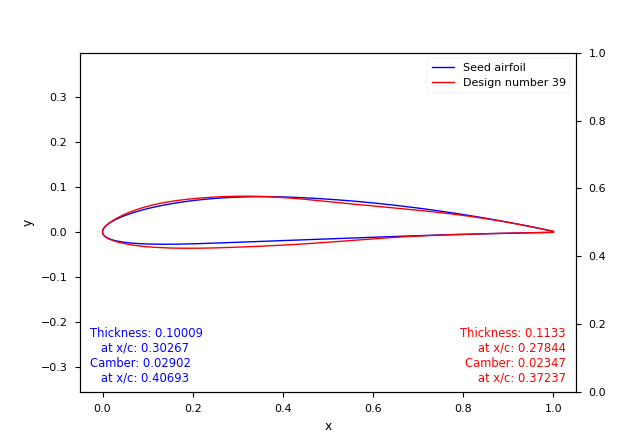
\includegraphics[width=0.49\textwidth]{User_Guide_figs/visualizer_foils.png}}
  \subfloat[Optimization history]{
    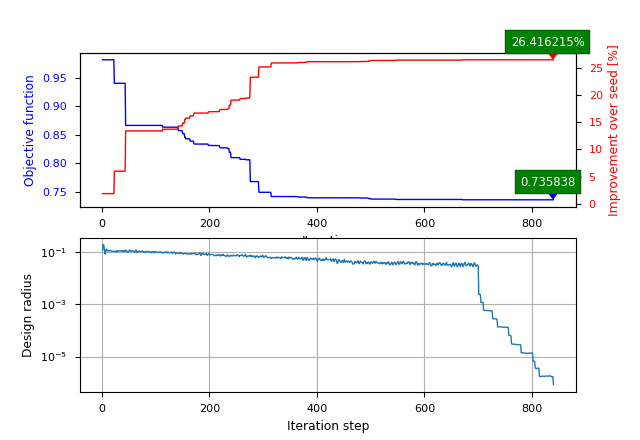
\includegraphics[width=0.49\textwidth]{User_Guide_figs/visualizer_progress.png}}

  \subfloat[Aerodynamics]{
    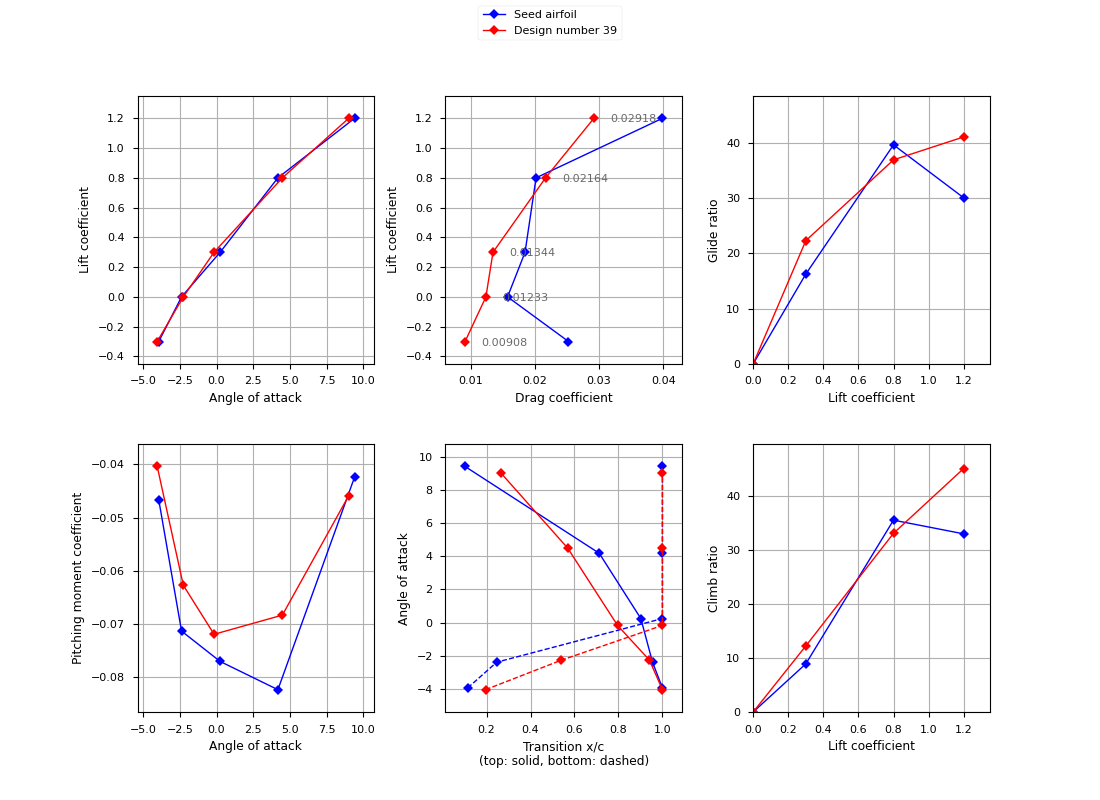
\includegraphics[width=0.75\textwidth]{User_Guide_figs/visualizer_aero.png}}
\caption{Example of plots generated by xoptfoil\_visualizer\_V2.}
\label{fig:visualizer_plot}
\end{figure}

\section{Using xfoil\_only}

Not available in this version.

Xoptfoil comes with a tool called xfoil\_only, which does exactly what it sounds like it
does: it runs Xfoil alone without optimizing. This can be useful for getting an idea of
how your seed airfoil will perform before optimizing, for example, or for checking the
performance of the optimized airfoil after the optimization. xfoil\_only uses the same
input file as Xoptfoil, except that many of the inputs are ignored. The relevant
inputs are the seed airfoil inputs (which is the one that will be analyzed), the operating
points, and the Xfoil settings. Note that if use\_flap is enabled, any flap angles 
specified in the operating\_conditions namelist will be applied, even if flap\_selection
is `optimize.' 

When xfoil\_only is run, it will first echo the options in the input file. If you have
disabled silent\_mode in the Xfoil options, Xfoil will print a lot of output to the screen
as it does its calculations. Finally, a summary of the geometric and aerodynamic info for
the airfoil will be displayed. If the calculations don't converge for any of the operating
points, a warning will be shown along with the aerodynamic results.

\section{Frequently asked questions}

There is a file called FAQ that is included in the Xoptfoil release. You can find answers
to frequently asked questions there.

\section{Example cases}

Two example cases with full input files and plots of the outputs can be in the
doc/example\_case directory included in the Xoptfoil release. There is also a file in
doc/ called `all\_inputs.txt,' which contains all of the possible inputs with comments.
It can be used as a template input file if desired; just be aware that many of the inputs
may not be needed or appropriate for every case.

\end{document}
